\documentclass{beamer}
%\documentclass[xcolor=dvipsnames]{beamer}
\usepackage[spanish]{babel}
\usepackage[utf8]{inputenc}
\usepackage{graphicx}
\usepackage{latexsym}

\newcommand{\beamer}{\textsc{beamer}}
\newtheorem{definicion}{Definición}
\newtheorem{ejemplo}{Ejemplo}

%%%%%%%%%%%%%%%%%%%%%%%%%%%%%%%%%%%%%%%%%%%%%%%%%%%%%%%%%%%%%%%%%%%%%%%%%%%%%%%
\title[Trabajo de Fin de Grado]{CodeLab\\
A Tool to automate repository creation and access control, giving support to distribute starter code, collect assignments and evaluate the students work on GitHub.}

\author[Samuel Ramos Barroso] {
Autor: Samuel Ramos Barroso \\
Director: Casiano Rodríguez León
}

\institute[ULL]{Escuela Superior de Ingeniería y Tecnología \\
                Departamento de Ingeniería Informática y de Sistemas \\
                Universidad de La Laguna}
\date[14-06-2018]{14 de Junio de 2018}
%%%%%%%%%%%%%%%%%%%%%%%%%%%%%%%%%%%%%%%%%%%%%%%%%%%%%%%%%%%%%%%%%%%%%%%%%%%%%%%

%\usetheme{Berlin}
\usetheme{Madrid}

%%%%%%%%%%%%%%%%%%%%%%%%%%%%%%%%%%%%%%%%%%%%%%%%%%%%%%%%%%%%%%%%%%%%%%%%%%%%%%%
\definecolor{pantone254}{RGB}{92,6,140}
\definecolor{pantone3015}{RGB}{92,6,140}
\definecolor{pantone432}{RGB}{92,6,140}
\setbeamercolor*{palette primary}{use=structure,fg=white,bg=pantone254}
\setbeamercolor*{palette secondary}{use=structure,fg=white,bg=pantone3015}
\setbeamercolor*{palette tertiary}{use=structure,fg=white,bg=pantone432}
\setbeamercolor*{palette sidebar primary}{use=structure,fg=pantone254}
\setbeamercolor*{palette sidebar tertiary}{use=structure,fg=pantone3015}
\setbeamercolor*{block title}{bg=pantone3015,fg=white}
\setbeamercolor*{alerted text}{fg=pantone432}
\setbeamercolor*{item projected}{fg=pantone254}
\setbeamercolor*{section in toc shaded}{use=structure,fg=structure.fg}
\setbeamercolor*{section in toc}{fg=pantone3015}
\setbeamercolor*{subsection in toc shaded}{fg=pantone3015}
\setbeamercolor*{subsection in toc}{fg=pantone432}

%%%%%%%%%%%%%%%%%%%%%%%%%%%%%%%%%%%%%%%%%%%%%%%%%%%%%%%%%%%%%%%%%%%%%%%%%%%%%%%
\begin{document}
  
%++++++++++++++++++++++++++++++++++++++++++++++++++++++++++++++++++++++++++++++  
\begin{frame}

  \includegraphics[width=0.3\textwidth]{img/ull.eps}
  \hspace*{7.5cm}
  \titlepage

\end{frame}
%++++++++++++++++++++++++++++++++++++++++++++++++++++++++++++++++++++++++++++++  

%++++++++++++++++++++++++++++++++++++++++++++++++++++++++++++++++++++++++++++++  
\begin{frame}
  \frametitle{Índice}  
  \tableofcontents
\end{frame}
%++++++++++++++++++++++++++++++++++++++++++++++++++++++++++++++++++++++++++++++  

\section{Introducción}
\begin{frame}[allowframebreaks,fragile]
  \frametitle{Introducción}
  
  \begin{center}

    CodeLab es una plataforma web basada en Javascript destinada al apoyo del profesorado para la realización de prácticas 
    intentando resolver las limitaciones que tienen otras plataformas para la gestión de prácticas.  

    \begin{figure}[!htb]  
      \minipage{0.32\textwidth}%
        
\includegraphics[width=\linewidth]{img/codelablogo.eps}
      \endminipage
    \end{figure}

  \end{center}

  \framebreak
  %+++++++++++++++++++++++++++++++++++++++++++++++++++++++++++++++++++++++++++++++++++++++++++++++++++++++++++++++++++++++++++++++++++++++++++
  
    CodeLab es similar en objetivos y funcionalidades a una herramienta desarrollada por GitHub: GitHub Classroom.  Github Classroom forma parte de Github Education:
  
  \begin{itemize}
    \item GitHub Classroom
    \item Classroom Desktop
    \item Teachers Pet (abandonado)
    \item Student Pack
  \end{itemize}

  \begin{figure}[!htb]  
    \minipage{0.32\textwidth}%
      
\includegraphics[width=0.7\linewidth]{img/classroom.eps}
    \endminipage
  \end{figure}

  \framebreak
    %+++++++++++++++++++++++++++++++++++++++++++++++++++++++++++++++++++++++++++++++++++++++++++++++++++++++++++++++++++++++++++++++++++++++++++
    GitHub Classroom simplifica la asignación de tareas, automatizando la creación de repositorios.
    Es una herramienta útil y sencilla de usar, tanto para profesores como para alumnos, 
    pero tiene ciertos defectos:

    \begin{itemize}
      \item No da soporte al proceso de evaluación 
      \item No se contempla el uso de Servicios de Integración Contínua como Travis para la evaluación de las pruebas
      \item Tiene un sistema para asociar información a cada alumno que es bastante limitado
    \end{itemize}

  \framebreak
  %+++++++++++++++++++++++++++++++++++++++++++++++++++++++++++++++++++++++++++++++++++++++++++++++++++++++++++++++++++++++++++++++++++++++++++
  
    CodeLab simplifica la asignación de tareas, automatizando la creación de repositorios.
  \begin{itemize}
    \item En CodeLab el profesor podrá crear tareas que serán asignadas a sus alumnos de forma individual o grupal. 
    \item Cada alumno o equipo realizará su trabajo en el repositorio git creado por CodeLab. 
    \item Una vez finalizado el trabajo, podrá ser revisado por el profesor.
    \item CodeLab provee mecanismos que dan soporte a la evaluación de las prácticas
  \end{itemize}

\end{frame}
  %+++++++++++++++++++++++++++++++++++++++++++++++++++++++++++++++++++++++++++++++++++++++++++++++++++++++++++++++++++++++++++++++++++++++++++

%  \framebreak
%  %+++++++++++++++++++++++++++++++++++++++++++++++++++++++++++++++++++++++++++++++++++++++++++++++++++++++++++++++++++++++++++++++++++++++++++
%  
%  En los últimos años se han desarrollado las nuevas tecnologías, lo que ha permitido que lleguen 
%  nuevas herramientas de aprendizaje y de apoyo a la docencia. Es el caso de la exitosa plataforma 
%  Moodle, un LCMS, sigla de Learning Content Management System.
  

\section{Objetivos}
\begin{frame}[allowframebreaks,fragile]
  \frametitle{Objetivos}
  
  Estos fueron los objetivos de este trabajo:

  \begin{itemize}
    \item Analizar otras plataformas  web existentes para la gestión del código de las prácticas de informática y su metodología de trabajo.
    \item Estudiar el funcionamiento de otras plataformas  web existentes para la gestión del código de las prácticas de informática.
    \item Estudiar las tecnologías a usar y enfocar el diseño de la plataforma web.
    \item Estudiar las funcionalidades que se van a incluir en la plataforma web.
  \end{itemize}

  \framebreak

  \begin{itemize}
    \item Crear una aplicación web básica que permita al usuario iniciar sesión con su cuenta de Github.
    \item Continuar con el desarrollo de la aplicación incluyendo las funcionalidades que solucionen las dificultades de otras plataformas  web existentes para la gestión del código de las prácticas de informática.
    \item Diseñar y desarrollar los estilos de las vistas.
  \end{itemize}
  
\end{frame}

%++++++++++++++++++++++++++++++++++++++++++++++++++++++++++++++++++++++++++++++  

\section{Tecnologías usadas}
\begin{frame}[allowframebreaks,fragile]
  \frametitle{Tecnología usada}
  
  Se escogió Express.js, Node.js y Javascript como tecnologías principales a usar en este proyecto 
  por las siguientes razones:

  \begin{itemize}
    \item Express.js es bastante fácil de aprender y usar.
    \item Se usa JS tanto en Backend como en frontend, ahorrando tiempo de desarrollo.
    \item El gestor de paquetes NPM.
  \end{itemize}

  \begin{figure}[!htb]
    \minipage{0.32\textwidth}
      
\includegraphics[width=\linewidth]{img/express.eps}
    \endminipage\hfill
    \minipage{0.32\textwidth}%
      
\includegraphics[width=\linewidth]{img/npmlogo.eps}
    \endminipage
  \end{figure}

  \framebreak

  Otras tecnologías usadas:

  \begin{itemize}
    \item Github API
    \item MongoDB - Mongoose
    \item Pug.js
    \item Materialize
  \end{itemize}

  \begin{figure}[!htb]
    \minipage{0.32\textwidth}
      
\includegraphics[width=0.7\linewidth]{img/github_ogo.eps}
    \endminipage\hfill
    \minipage{0.32\textwidth}%
      
\includegraphics[width=0.7\linewidth]{img/mongo.eps}
    \endminipage    
    \minipage{0.32\textwidth}%
      
\includegraphics[width=0.7\linewidth]{img/pug.eps}
    \endminipage
  \end{figure}
\end{frame}

%++++++++++++++++++++++++++++++++++++++++++++++++++++++++++++++++++++++++++++++

\section{Desarrollo de la plataforma}
\begin{frame}
\frametitle{Desarrollo de la plataforma}
  
  \begin{center}
    \includegraphics[width=0.8\textwidth]{img/codelab.eps}
  \end{center}

\end{frame}

\subsection{Github API}
\begin{frame}
\frametitle{Github API}
  
  Para poder usar Github como estructura para la creación de aulas y tareas de código usaremos 
  la Github REST API V3. La API permite acceder a las funcionalidades de Github, 
  A continuación se detallará que funcionalidades de la Github API se han usado

  \begin{itemize}
    \item OAuth
    \item Organizaciones, repositorios y equipos.
  \end{itemize}

  \begin{figure}[!htb]  
    \minipage{0.32\textwidth}%
      
\includegraphics[width=\linewidth]{img/octokit.eps}
    \endminipage
  \end{figure}
  
\end{frame}
  %+++++++++++++++++++++++++++++++++++++++++++++++++++++++++++++++++++++++++++++++++++++++++++++++++++++++++
  
\subsubsection{OAuth}
  
\begin{frame}
\frametitle{OAuth}

  Desde el punto de vista de Codelab, OAuth proporciona un método de acceso a los datos de Github 
  a la vez que se protegen los credenciales de la cuenta. Solicitamos al usuario una serie de 
  accesos y permisos en sus datos, para poder operar con las organizaciones y repositorios de Github.
  
  \begin{figure}[!htb]  
    \minipage{0.32\textwidth}%
      \includegraphics[width=1.2\linewidth]{img/oauth.eps}
    \endminipage
  \end{figure}

\end{frame}
  %+++++++++++++++++++++++++++++++++++++++++++++++++++++++++++++++++++++++++++++++++++++++++++++++++++++++++++
  
\subsubsection{Organizaciones repositorios y equipos}

\begin{frame}
\frametitle{Organizaciones repositorios y equipos}

  Las operaciones que realizaremos con Organizaciones, repositorios y equipos son las siguientes:

  \begin{itemize}
    \item Obtener las organizaciones del usuario.
    \item Añadir usuarios a la organización.
    \item Crear un repositorio en las organizaciones.
    \item Añadir colaboradores al repositorio.
    \item Crear equipos.
    \item Añadir un equipo a un repositorio.
    \item Comprobar si un usuario es miembro de un equipo.
    \item Obtener los repositorios de una organización.
    \item Crear un fichero en un repositorio.
  \end{itemize}

\end{frame}

%++++++++++++++++++++++++++++++++++++++++++++++++++++++++++++++++++++++++++++++  
  
\subsection{MVC}

\begin{frame}
\frametitle{MVC}

  El modelo vista controlador es una arquitectura de software que separa la lógica de
  la aplicación de la interfaz de usuario. Lo hace separando la aplicación en tres partes: 
  el modelo, la vista y el controlador.   

   \begin{figure}[!htb]  
    \minipage{0.32\textwidth}%
      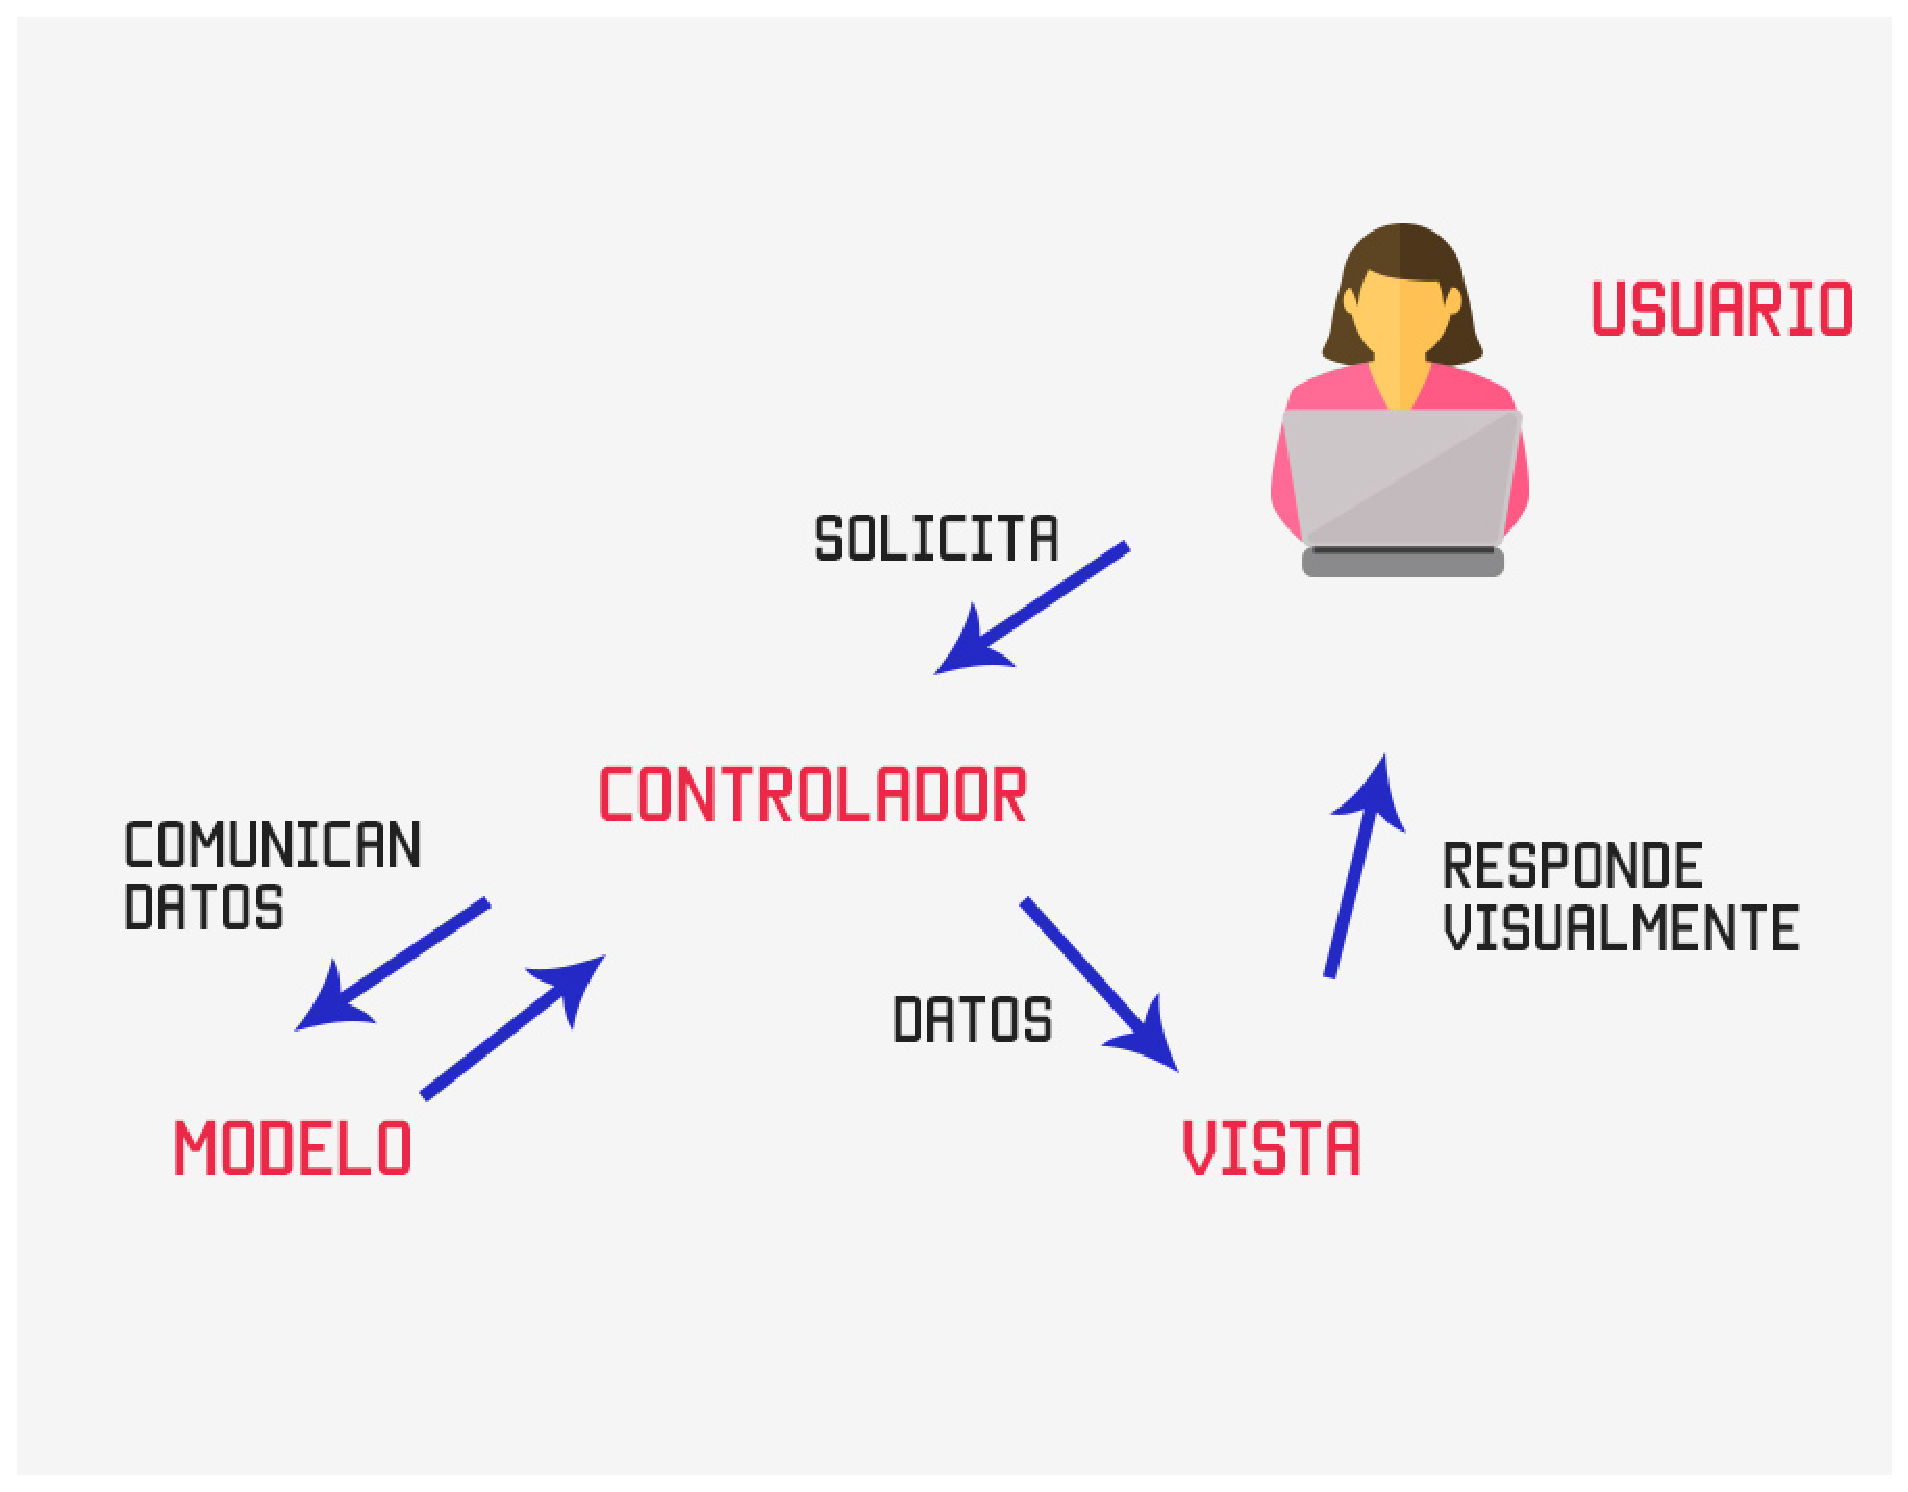
\includegraphics[width=\linewidth]{img/29.eps}
    \endminipage
  \end{figure}

\end{frame}

%+++++++++++++++++++++++++++++++++++++++++++++++++++++++++++++++++++++++++++++++++++++++++++++++++++++++++++

\subsection{Diseño de la base de datos}

\begin{frame}[allowframebreaks]
\frametitle{Diseño de la base de datos}

  Se usará una base de datos NoSQL, en concreto MongoDB como sistema gestor y Mongoose como ODM, 
  por lo que nos referimos las tablas como colecciones, columnas como claves y filas como objeto.
  
  \bigskip
  
  La base de datos es una parte muy importante de la plataforma, ya que en ella recae toda 
  la responsabilidad de simular toda la estructura de aulas y tareas.

   \begin{figure}[!htb]  
    \minipage{0.32\textwidth}%
      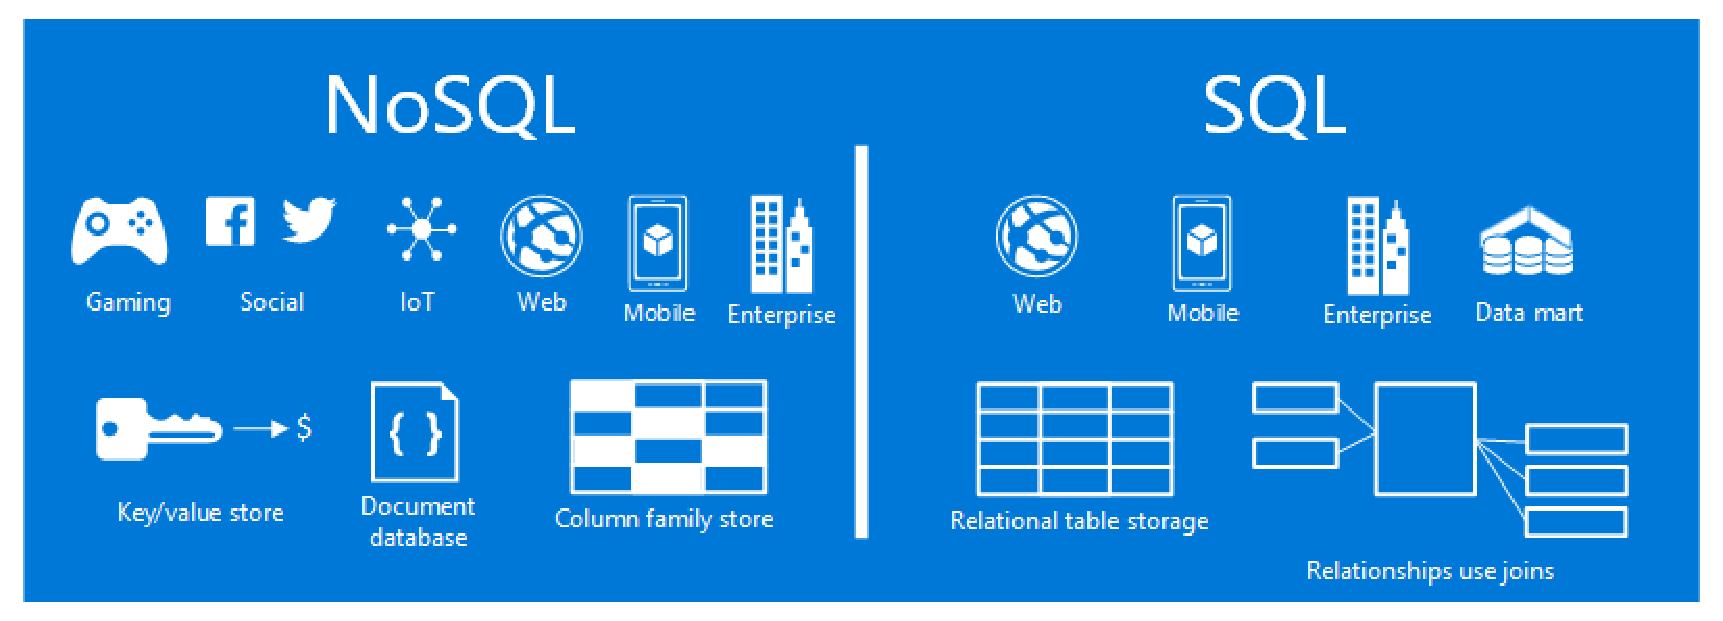
\includegraphics[width=1.2\linewidth]{img/nosql.eps}
    \endminipage
  \end{figure}

  \framebreak

    Las colecciones son las siguientes:

    \begin{itemize}
      \item Usuarios
      \item Organizaciones
      \item Asignaciones
      \item Asignaciones en grupo
      \item Asignaciones individuales
      \item Equipos
      \item Alumnos
    \end{itemize}

\end{frame}

%+++++++++++++++++++++++++++++++++++++++++++++++++++++++++++++++++++++++++++++++++++++++++++++++++++++++++++

\section{Funcionalidades}

\begin{frame}[allowframebreaks]
\frametitle{Funcionalidades}

  El proyecto se divide en tres paquetes de funcionalidades, Cada paquete incluye funcionalidades para cada rol:

  \begin{itemize}
    \item Funcionalidades básicas
    \item Funcionalidades para profesores.
    \item Funcionalidades para el alumno
  \end{itemize}

  \framebreak
  
  Las funcionalidades básicas son comunes a todos los roles que participan en la plataforma, 
  tanto alumnos como profesores, todos pueden hacer Log in, Log out y consultar un perfil.
  
  \bigskip
  
  Como alumno el usuario puede visitar el perfil, donde encontrará información básica de Github y dos pestañas, 
  en las que el alumno tiene un historial de las tareas que ha realizado de forma grupal e individual.
  
  \bigskip

  Los profesores tendrán el grupo de funcionalidades más completo, ya que ellos son los protagonistas 
  de la app.

  \framebreak

  Los profesores podrán desempeñar las siguientes tareas:

  \begin{itemize}
    \item Añadir una organización como aula.
    \item Invitar alumnos al aula.
    \item Crear una tarea.
    \item Añadir un fichero de alumnos asociado al aula.
    \item Editar las opciones del aula.
    \item Invitar alumnos a la tarea.
    \item Editar las opciones de la tarea.
    \item Crear un repositorio de evaluación de cada tarea.
  \end{itemize}

\end{frame}

%+++++++++++++++++++++++++++++++++++++++++++++++++++++++++++++++++++++++++++++++++++++++++++++++++++++++++++
  
\section{Caso de uso}

\begin{frame}[allowframebreaks]
\frametitle{Caso de uso}

  Con vistas a probar y testear que todo funcionaba de forma correcta, Casiano me sugirió probar 
  la plataforma para la realización de algunas prácticas individuales y grupales. Por ello, decidimos 
  realizar algunas tareas para la asignatura de Procesadores de Lenguajes en CodeLab.

  \framebreak

  \begin{figure}[!htb]
      \includegraphics[width=\linewidth]{img/gh.eps}
  \end{figure}

  \framebreak

  \begin{figure}[!htb]
      \includegraphics[width=\linewidth]{img/teams.eps}
  \end{figure}

  \framebreak

  \begin{figure}[!htb]
      \includegraphics[width=\linewidth]{img/campus.eps}
  \end{figure}

\end{frame}

%+++++++++++++++++++++++++++++++++++++++++++++++++++++++++++++++++++++++++++++++++++++++++++++++++++++++++++

\section{Conclusions and Future Work}
\begin{frame}[allowframebreaks]
  \frametitle{Conclusions and Future Work}

  \begin{itemize}
    \item CodeLab was born as a tool that aims to extend the functionality of other tools such as Github 
          Classroom, adding specific functions for the teachers to support the management of courses and 
          the correction of programming labs.
    \item The platform has been designed with ease of use in mind for those who are not familiar with GitHub.
    \item Version control offers many advantages to developers. Most development companies use the git 
          version control system, and consequently it is essential that students learn to handle git correctly.
  \end{itemize}
  \framebreak
  %+++++++++++++++++++++++++++++++++++++++++++++++++++++++++++++++++++++++++++++++++++++++++++++++++++++++++++++++++++++++++++++++++++++++++++
  
  {\bf Future Work:}
  \begin{itemize}
    \item I would like to continue developing CodeLab, improving it and adding new functionalities. 
    \item One of the first improvements that is proposed is the use of a front-end library such as Vue 
          or React to improve the visual quality of the web platform.
    \item A new functionality that I would like to add is the possibility of more than one teacher per classroom.
  \end{itemize}
\end{frame}

%++++++++++++++++++++++++++++++++++++++++++++++++++++++++++++++++++++++++++++++ 

\section{Bibliografía}
\begin{frame}[allowframebreaks]
  \frametitle{Bibliografía}
  \bibliographystyle{ieeetr}
  \bibliography{presentacion_tfg}
  \nocite{*}
\end{frame}

\begin{frame}
  \frametitle{Fin de la presentación}
  \begin{center}
    \Huge{Gracias por su atención}
  \end{center}
\end{frame}

\end{document}
